\chapter{Résultats et discussions}

\newthought{Le dispositif technologique} que nous avons choisi de développer permet d'observer dans le détail la diffusion de mèmes ou autres formes de contenus identifiés sous la forme d'un ensemble de messages. Les expérimentations préliminaires nous permis de constater que la détection des mèmes était une tâche peu aisée. Ainsi, nous allons décrire ici l'approche que nous avons choisi de retenir (choix technologiques, algorithmes et processus de validation). Utilisant la recherche par mots-clés pour constituer un corpus de messages, notre outil permet ensuite d'extraire et d'analyser ces données pour observer les dynamiques qui l'entoure. Après avoir détaillé son fonctionnement et interface, nous présenterons un ensemble de résultats obtenus grâce obtenus grâce à un échantillon d'une douzaine de mèmes. Après avoir considéré comment ces résultats nous informe sur les différents types et formes de contenus, nous discuterons des limites, contraintes et écueils possibles d'une approche utilisant l'analyse de données.

\subsubsection{A propos des choix technologiques}

    Nous avons été amené à effectuer de nombreux choix quant aux outils utilisés. Chacun des logiciels, programmes ou outils mobilisés sera présentés plus en détail dans les sections ci-dessous. Néanmoins, afin d'éclaircir le lecteur sur la nature et les raisons plus générales de ces choix, nous précisons ici les différents aspects qui sont entrés systématiquement en compte lors de chacune de  nos décisions :

    \begin{description}
        \item[Licence : gratuité, open-source et disponibilité]
            La possibilité de lire, modifier et utiliser les outils et librairies dans le cadre de cette recherche est un des éléments primordiaux. Non seulement, les coûts de développement sont très largement diminués par l'usage de solutions gratuites mais également la disponibilité des outils permet à ceux qui le souhaiterait de se réapproprier le code librement. De plus, le caractère \textit{open source} permet de consulter librement les rouages du code et s'assurer de sa validité et sa qualité avant de l'invoquer.

        \item[Documentation : communauté et support]
            Les outils parfois compliqués du développement informatique ne peuvent souvent être utilisés sans un minimum d'explication et de documentation. Si la documentation laisse à désirer, que le code est mal rédigé ou que la communauté des créateurs ou utilisateurs n'est pas présente procurer des explications, l'usage de technologies même très intéressante devient très difficile, voire impossible. Ainsi, nous avons opté pour des solutions possédant une documentation satisfaisante afin de simplifier leur ré-utilisation .

        \item[Interopérabilité : déploiement et compatibilité]
            Le degré de complexité des procédures d'installation et de mise en place est également un facteur décisif dans la sélection d'un outil. En effet, la reproductibilité et la possibilité de réutilisation du code se voit très largement diminuée par un déploiement complexe et laborieux, multipliant souvent les erreurs. Les outils choisis pour ce travail ont été développé pour être compatibles avec le système d'exploitation Linux Debian, très largement répandu.

        \item[Validation : usage commercial et scientifique]
            Notre recherche ne se situe pas dans le domaine de la science informatique. \'A ce titre fait usage d'outils utilisés tant dans la communauté scientifique que dans l'industrie du Web. Le développement de nombreux  outils commerciaux s'originent dans la recherche scientifique. L'optimisation et la validation du code par les processus de contrôle de qualité de l'industrie sont également un facteur important dans la décision d'utiliser telle ou telle technologie.
    \end{description}

    L'ensemble de ces raisons nous a porté à utiliser le langage \textit{Python} comme principal outil de développement de notre outil. Largement utilisé par la communauté scientifique, Python dispose de nombreuses librairies, plugins et outils qui le rendent attractif et efficace pour le prototypage et la recherche scientifique. De nombreux outils statistiques pour l'analyse de données ainsi que la plupart des algorithmes récents sont maintenus dans le package \textit{SciPy}. Également, il est simple a déployer et possède de nombreuses ressources pour aider au développement et à la documentation.

\section{Un outil de traitement et de visualisation des mèmes}

    Dans cette section, nous présenterons la structure et les développements spécifiques que nous avons mené pour construire cet outil. Les comment et pourquoi de nos différents choix technologiques seront explicités dans une présentation pas à pas du fonctionnement et de l'utilisation du système d'analyse que nous avons créé.

\subsection[Constitution de corpus par mots-clés pour chaque mème]{Constitution de corpus par mots-clés pour chaque mème}
    \label{sec:keywords}

    Comme nous l'avons vu précédemment,  ni les méthodes de détection algorithmiques (section \ref{sec:protomemes}) ni l'usage de l'objet hashtag (section \ref{sec:hashtags}) n'ont permis de saisir de manière satisfaisante l'objet mème dans le vaste jeu de données que nous avons choisi d'approcher (section \ref{sec:weiboscope}). 

    Ainsi, nous avons choisi de considérer l'approche lexicale qui consiste à décrire le mème sous la forme de mots-clés. Pour chaque mème, nous procédons à l{\textquoteright}extraction d{\textquoteright}un jeu de données contenant l{\textquoteright}ensemble des messages correspondant à une requête définie composée de différents mots. 

    La faiblesse intrinsèque de cette approche est néanmoins qu'elle nécessite de savoir ce qu'on veut chercher, à l'inverse d'une détection des mèmes qui permettrait de les identifier sans connaître leur existence a priori. Cette méthode prend peu en compte les éléments audio et visuels (images, vidéos) qui constituent pourtant une partie importante des mèmes constitués en ligne. 

    Néanmoins, elle permet une approche intuitive par l'usage de mots-clés et une vérification itérative de la qualité des résultats obtenus, à l'inverse de la détection algorithmique notamment. Également, les faiblesses de la recherche plein-texte peuvent être contournées relativement facilement (effacement des éléments exogènes, complétion des corpus). 

\subsubsection[Indexation pour la recherche plein-texte]{Indexation du corpus Weiboscope pour la recherche plein-texte}

    La fonction de recherche plein-texte est un des secteurs des technologies numériques qui a connu la plus forte expansion depuis les 10 dernières années de l'Internet, comme en témoigne l'histoire de \textit{Google}. L'accroissement des données et la nécessité de naviguer en leur sein ont fait des moteurs de recherche un élément incontournable du paysage de nos navigateurs. Chaque site web possède un champ "search" ou presque. Suivant cet important développement, des solutions de plus en plus fiables et performantes ont été mis à disposition sous des licences ouvertes, permettant facilement une appropriation.

    Dans cette étude, nous avons choisi d'utiliser le moteur de recherche \textit{ElasticSearch}\footnote{Voir le site \url{http://www.elasticsearch.org}, consulté le 22 Avril 2014 à 12:23} pour accéder au contenu du corpus. Utilisant la très solide technologie du  moteur d'indexation \textit{Apache Lucene}  \footnote{ \url{http://lucene.apache.org/} consulté le 20 Juin 2014 à 11:22}, il permet d'indexer de larges corpus dans une base de données non-relationnelles, mettant à disposition une API efficace et structurée suivant la norme \textit{REST}. Largement utilisé et documenté, \textit{ElasticSearch} permet l'indexation des caractères chinois grâce au plugin Lucene \textit{SmartChinese Analyzer}. Ce plugin utilise un algorithme basé sur le modèle statistique dit de \textit{Modèle de Markov caché} appliqué à un vaste \textit{training corpus} de texte Chinois et de dictionnaires\footnote{Voir \url{http://www.ictclas.org/} consulté le 7 Juillet 2014 à 11:32} pour segmenter le texte chinois en mots. Les mots sont ensuite indexés dans la base de données de \textit{Lucene}. Chaque requête dans \textit{ElasticSearch} permet de comparer les instructions (mots-clés) aux documents textuels contenu dans la base de données, attribuant un poids spécifique à chaque document en fonction de la corrélation entre ses mots et ceux de la requête. Enfin, le moteur de recherche renvoie les résultats sous la forme d'un objet au format standard JSON qui permet sa réutilisation dans une interface pour l'interprétation des résultats obtenus.

    Afin de procéder à la recherche de mème dans le texte, nous avons donc indexé dans \textit{ElasticSearch}les parties du corpus \textit{Weiboscope} à l'aide d'un script\footnote{consultable ici \url{https://github.com/clemsos/mitras/blob/master/es_build_index.py} consulté le 7 Juillet 2014 à 11:27}. Chacun des 52 fichiers au format \textit{zip} contenant des données au format \textit{csv} (texte des microblog en chinois et méta-données)  peut donc être déposé dans un dossier sélectionné pour être ensuite indexé. Cette manipulation est également reproductible pour tout type de fichiers en langue chinoise ou anglaise (d'autres langues nécessite l'ajout d'un simple analyseur de texte \textit{Apache Lucene}).

\subsubsection[Sélection qualitative de mots-clés]{Sélection qualitative de mots-clés}

    Une fois le texte indexé, il nous faut maintenant définir les requêtes appropriés qui nous permettront d'extraire un corpus intéressant pour l'étude d'un ou plusieurs mèmes. La définition des mots-clés est un exercice compliqué dans de nombreux cas car il suppose que les mèmes ne recoupent pas ou peu des mots utilisés dans des sens multiples. Or, nous avons vu que le propre du mème est justement l'intertextualité et à ce titre joue littéralement sur les mots. Dans le contexte chinois, nous avons notamment vu l'exemple d'un mème construit autour des mots \textit{crabe de rivière} (voir figure \ref{fig:hexie}). Il y a de très fortes chances que les résultats d'un recherche pour les mots \textit{crabe} et \textit{rivière} dans le moteur de recherche et peu de lien avec ce mème somme toute très marginal dans la masse des contenus. Ici, la syntaxe propre du moteur de recherche peut nous venir en aide, permettant d'inclure (\textit{AND}) ou d'exclure (\textit{NO}) certains mots précis ou d'exiger du moteur de considérer des groupes de mots entier \textit{""}. Une autre possibilité est de limiter la recherche dans le temps en se concentrant sur une période donnée où le  mème connaît sa période de plus fort intérêt.

    La qualité de la requête et des résultats renvoyés par le moteur de recherche pour chaque mème peut se définir  selon trois aspects importants :

    \begin{description}
        \item[volume]
            Taille significative et volume suffisant de données pour constituer un corpus représentatif du mème.
        \item[qualité]
            Possibilité de vérifier manuellement la qualité du contenu par la lecture d{\textquoteright}un échantillon de  messages obtenus.
        \item[dimensions]
            Les différents paramètres retournés (dates, lieu, utilisateur précis, contenu censuré...) correspondent à ceux choisis dans la requête
    \end{description}

    La définition de la requête répondant au mieux aux besoins du chercheur  ne peut donc se faire a priori sans un certain nombre d'essais et tentatives. L'obtention de résultats satisfaisants passe par une phase itérative qui permet de définir et cerner une définition du mème sous forme d'une requête dans le moteur de recherche. Cette démarche implique non seulement la possibilité de pouvoir s'adonner à de multiples essais de formulations de la requête mais également la nécessité de lire les résultats sous une forme compréhensible. Si le format JSON reçu ou renvoyé par le moteur de recherche est un standard de l'échange de données, il n'est néanmoins pas adapté à la lecture et l'écriture par des humains. Ainsi, afin de pouvoir mener ce travail de façon intuitive et pratique, nous avons mis en place un tableau de bord à l'aide du logiciel \textit{Kibana} qui nous permet de contr\^oler la pertinence des résultats en comparant plusieurs requêtes différentes.

    \begin{figure}[h!]
        \centering
        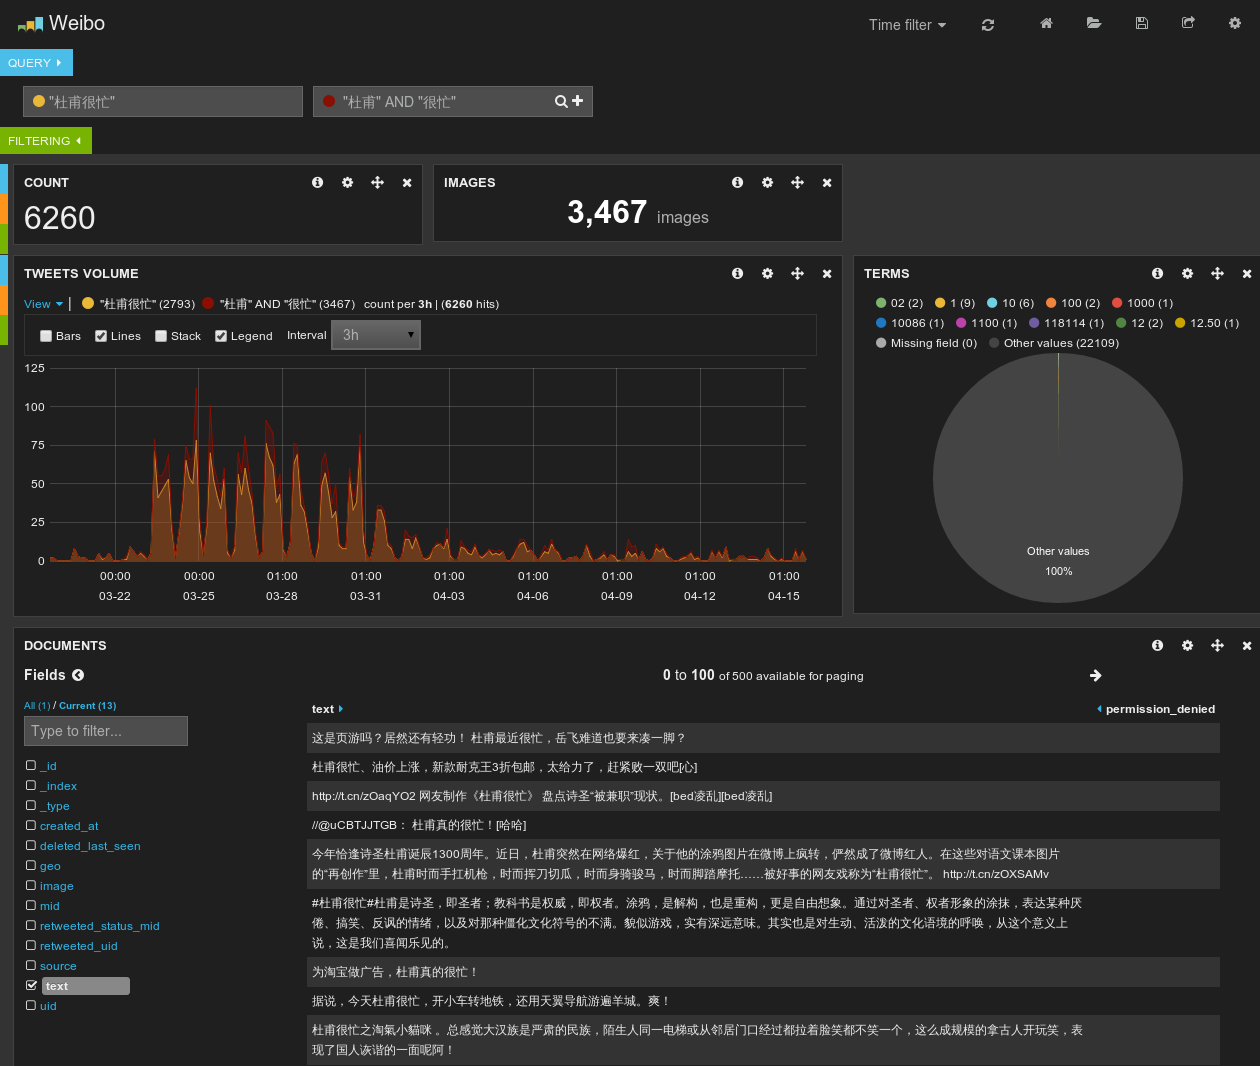
\includegraphics[width=6.0004in,height=5.078in]{figures/chap4/ui/ui-kibana.png}
        \caption[Tableau de bords requêtes par mots-clés] { Ce tableau de bord permet de comparer la qualité de différentes requ\^etes dans le corpus. Capture d'écran réalisée le 23 Mars 2014 à 16h18}
    \end{figure}

\subsubsection[Constitution d'un corpus pour chaque mème]{Constitution d'un corpus pour chaque mème}

    En contrôlant la qualité de ses différents critères nous pouvons donc identifier une requête adéquate pour décrire le mème. Une fois cette étape effectuée, nous procédons à l'extraction des messages qui vont venir constituer le corpus d'études de notre mème. Pour s'assurer de la fiabilité des résultats, nous disposons de l'index de poids du moteur de recherche qui représente la similarité entre notre requête et les messages obtenus. Pour limiter le nombre de résultats, nous pouvons fixer un poids minimum (par exemple 0,5) et ainsi limiter le bruit en ignorant les messages sans lien avec notre requête.

    Une fois extrait, ce jeu de données est stocké dans un fichier de type  \textit{csv} respectant le format initial et l'encodage des données de Weiboscope. Afin de parfaire la complétude de ce jeu de données, les messages mentionnés et les retweets ne contenant pas le mot clé (commentaires, réponses, etc.) sont rassemblés pour donner finalement un ensemble de messages représentatifs du mème qui va pouvoir être étudié.


\subsection[Analyse des graphes et traitement des données]{Analyse des graphes et traitement des données}

    Une fois les corpus pour différents mèmes extraits, nous pouvons procéder à l'analyse. Il s'agit donc pour nous d'observer plusieurs aspects importants de la diffusion des mèmes : champ sémantique, dynamique des discussions et dimension actuelle et localisée de ces échanges. Principalement, nous choisissons de représenter différents réseaux sémantiques, conversationnels et géographiques qu'ils s'agit d'extraire du corpus de message des mèmes afin de les représenter. Nous souhaitons également  pouvoir observer les relations existantes entre ces différents réseaux présents lors de la diffusion. En effet, les croisements de ces différentes dimensions peuvent montrer les phénomènes les plus intéressantes, en ramenant de la géographie dans le langage où en affichant l'existence locale des conversations.

    Les choix méthodologiques de cette étude cherchent notamment à démontrer que les actes de communication ne peuvent simplement se comprendre comme des échanges {\textquotedblleft}sociaux{\textquotedblright} mais doivent être appréhendés plus largement comme des actes d{\textquoteright}énonciation complexes possédant de multiples dimensions sémantiques, temporelles, conversationnelles toutes localisées.

    Nous définissons ces trois dimensions comme suit :

    \begin{description}
        \item[Langagier]
        Le champ sémantique d{\textquoteright}un mème est constitué des mots qui sont prononcés lors de sa diffusion. L{\textquoteright}association de mots -souvent sous la forme du jeu de mots - est un des propres du mème et constitue ainsi une part importante de son existence. Ainsi, le mème produit à proprement parler des réseaux de mots en dessinant des liens entre des signifiants souvent improbables qui en font souvent le succès \citep{Bauckhage2011}. Observer les étapes de la construction du réseau de mots qui le constitue peut donc permettre un éclairage nouveau.

        \item[Conversationnel] 
        Plus que les mots, un mème se constitue sous la forme d{\textquoteright}un échange, une conversation o\`u les différents acteurs discutent, commentent et se saisissent des actions disponibles sur la pateforme web (like, retweets, etc.) pour converser. Comme nous l{\textquoteright}avons vu précédemment, nous pouvons identifier et considérer un graphe conversationnel créé par le mème en se diffusant pour identifier des structures de diffusion particulières. 

        \item[Réel] 
        Au-delà des échanges en ligne, ces discussions possèdent une existence physique, premièrement sous la forme de l{\textquoteright}activité électrique des machines qui sont utilisées lors de ce processus. Néanmoins, dans l{\textquoteright}approche d{\textquoteright}une géographie humaine des échanges numériques, nous considérerons ici l{\textquoteright}existence physique des mèmes par celle des utilisateurs - de leurs corps - et non pas des machines. 
    \end{description}

    Afin d{\textquoteright}étudier chacun de ces aspects du mème, nous allons donc procéder à la collection de connaissances sur chacun de ces aspects d'après le corpus de données du ou des mèmes sélectionnés. Nous procédons ensuite au traitement de chaque corpus selon une série de procédures que nous allons maintenant définir. 

\subsubsection[Traitement naturel de la langue chinoise]{Traitement naturel de la langue chinoise}

    Le texte de chaque message est analysé de fa\c{c}on à ne conserver que les éléments significatifs et utiles à l'analyse : mots importants, mentions d'utilisateurs, urls et hashtags. Les éléments propres à \textit{Sina Weibo} peuvent aisément être identifiés à l'aide d'expressions régulières car elles suivre des patterns stricts : 

    \begin{itemize}
     \item le hashtag débute et termine par le symbole \# (ex. \#hello\#)
     \item les urls suivent une forme stricte (ex. \url{http://t.cn/SVWAfP}) 
     \item les mentions d'utilisateurs débute normalement par $@$ suivi du noms de l'utilisateur mentionné. Le corpus Weiboscope ayant été anonymisé, le nom des utilisateurs a été remplacé par un identifiant commençant par la lettre \textit{u} suivi de 8 caractères (ex.$a$uY02ZFLAN)
    \end{itemize}


    Le texte rédigé présent dans les messages est par contre un élément beaucoup plus complexe à traiter. De plus, la langue écrite chinoise, contrairement aux langues de l'alphabet latin, n'utilise pas d'espace pour séparer les mots d'une phrase. Ainsi, alors qu'il est plutôt simple de repérer les différents mots d'une phrase en langue française ou allemande en recherchant les espaces dans le texte, la phrase chinoise nécessite d'être segmentée en mots avant de pouvoir être traitée. Le nom commun chinois prend  le plus souvent la forme d'une série de deux caractères mais de nombreux noms plus techniques, les noms propres et les verbes ne suivent pas cette logique. La segmentation de la phrase chinoise est donc une  première contrainte qu'il nous faut prendre en compte dans le cadre de cette étude, le chinois constituant le langage majoritaire de notre corpus. 

    Le domaine du \textit{Natural Language Processing} (NLP)) en chinois est un sujet de recherche encore très discuté \citep{Qiu2013}. De nombreuses solutions, librairies et logiciels sont disponibles pour la segmentation des phrases chinoises et l'identification de mots-clés notamment. Néanmoins, l{\textquoteright}identification de la meilleure option parmi la multitude des outils a constitué un des aspects préliminaires importants de notre travail d{\textquoteright}analyse de données. Nous avons bénéficié ici de l'aide de Yuan Mingli, directeur du centre de Recherche et Développement de la compagnie \textit{Guokr}\footnote{Voir le site officiel \url{http://www.guokr.com/} consulté le 5 Juillet à 15h45}. Situé à Beijing, \textit{Guokr} est un site ressource pour la culture scientifique en Chine qui propose notamment des cours en ligne et des listes de discussions sur de nombreux sujets en lien avec les sciences et les technologies. Une partie de l'équipe de recherche dédie son travail au développement et à la maintenance de solutions d'outils pour le Web chinois, notamment pour l'analyse naturelle de la langue chinoise. Ayant travaillé auparavant sur des dispositifs d'analyse de données avec Yuan Mingli dans le cadre du projet \textit{Sharism Lab}\footnote{\url{http://sharismlab.com}, consulté le 6 Juillet 2014 à 13h46}, nous nous sommes rendus à Pékin lors d'un séjour de recherche en Septembre 2013 pour identifier les solutions les plus intéressantes pour l'analyse de la langue chinoise.

    Nous avons ainsi réalisé un benchmark afin de comparer les différents algorithmes de segmentation existants et définir le plus approprié pour ce travail. Nous avons testées plusieurs solutions, dont plusieurs développés par l'équipe de \textit{Guokr} elle-même:  

    \begin{description}
        \item[gkSeg] 
        Cette solution utilise un algorithme appelé \textit{Conditional Random Fields} qui s'intéresse à chacun des caractères. Il est conçu pour pouvoir être utilisé aussi bien sur des  textes en chinois ancien\footnote{ gkSeg : \textit{{\textquotedblleft}Yet another Chinese word segmentation package based on character-based tagging heuristics and CRF algorithm{\textquotedblright} }\url{https://github.com/guokr/gkseg}, consulté le 14 Mars à 18:28}.

        \item[Stanford CoreNLP Chinese Segmenter]
        Le célèbre outil de NLP développé par Stanford dans sa version 3.4 permet de découper la phrase chinoise. La librairie \textit{stan-cn-seg}\footnote{\url{https://github.com/guokr/stan-cn-seg} consulté le 7 Juillet à 16:01} permet de l'utiliser simplement sous la forme d'un serveur.

        \item[neuseg]
        Ce protocole expérimental utilise les réseaux neuronaux et le modèle vectoriel pour segmenter la phrase chinoise\footnote{\url{https://github.com/guokr/neuseg} consulté }.

        \item[jieba]
        Jieba\footnote{ \url{https://github.com/fxsjy/jieba}, consulté le 14 Mars à 18:30} est un segmenteur open-source  très répandu et utilisé commercialement dans de nombreux projets. Plus généreux en termes de fonctionnalités, il permet de meilleures performances sur de larges corpus. Il utilise l'algorithme Trie tree pour recréer des \textit{directed acyclic graph} à partir des mots de la phrase. Les mots inconnus sont détectés grâce à l'algorithme \textit{Viterbi}.
    \end{description}

     Après plusieurs tentatives, nous avons préféré le segmenteur \textit{Jieba}, plus adapté que les solutions expérimentales dans le cas de notre large corpus. \textit{Neuseg} n'était pas assez mature et ne permettait pas d'obtenir des résultats satisfaisant, connaissant beaucoup d'erreurs et manquant de stabilité lors de l'usage . \textit{Standford NLP} nous contraignaient à l'usage d'un serveur externe rendant le déploiement plus complexe et l'ensemble plus compliqué à maintenir. \textit{Gkseg} ne présentait pas de performances suffisantes en terme de temps de traitement, devenant handicapant pour notre étude. De plus, \textit{Jieba} se présente sous la forme d'une librairie \textit{Python}, langage que nous avions choisi d'utiliser pour l'écriture de cet outil.

    \begin{algorithm}[h]
        \caption{Extract Words from Message}
        \label{algo:message-graph}
        \begin{algorithmic}

                \Require{$m$ is a microblog text message}
                \Require{$stopwords$ is a list of common words that should be excluded}
                \Require{\Call{Jieba NLP}{$text$} is a Chinese language word segmenter}
                \State $words \gets \Call{Jieba NLP}{$m$}$ segment the sentence
                \State remove $stopwords$ from $words$                

        \end{algorithmic}
    \end{algorithm}

    La phrase est donc segmentée  pour obtenir un ensemble de mots du mème. Néanmoins, de nombreux mots dans une phrase sont redondants ou inutiles pour décrire notre mème. Afin de s'intéresser seulement aux mots les plus importants, il est donc important de  supprimer les mots les plus communs, appelés \textit{stopwords}\footnote{La liste des mots ignorés (\textit{stopwords}) dans cette recherche est disponible en ligne à \url{https://github.com/clemsos/mitras/tree/master/lib/stopwords}}. La première forme de stopwords est celle propre à la langue chinoise. De nombreux mots très usités ne possèdent que peu d'information pour notre étude et peuvent donc être supprimés. Nous utilisons pour cela la fonctionnalité de \textit{Jieba} qui propose un dictionnaire comprenant caractères traditionnels et simplifiés et permet d'enlever les mots les plus courant. Une seconde liste de stopwords a été ajouté pour parfaire le tri des informations. Cette liste a été constituée lors du projet commercial \textit{Echidna} réalisé en Avril 2013 à Shanghai avec l'équipe constituée par Ricky Ng-Adam, ancien ingénieur à Google (Montain View, USA) pour le compte de la société \textit{Transist} (\zh{创思}). Echidna était une solution permettant de connaître les tendances par mots-clés en temps-réel sur le réseau Sina Weibo grâce à une infrastructure d'analyse de données et un tableau de bord. Lors de ce projet, de nombreux outils et concepts ont été dessinés, notamment en termes de communication entre les différentes parties du système. Une liste de stopwords a également été constituée au fur et à mesure de l'amélioration du système. Ce projet est aujourd'hui terminé mais la liste des stopwords a été réutilisée dans le présent travail.
    
\subsubsection{Graphe lexical}

    L'étape précédente nous a permis d'extraire l'ensemble des entités pour chaque message, dont notamment un ensemble de mots-clés. Afin d'étudier les relations existantes entre ces mots-clés, nous devons maintenant constituer le graphe sémantique du mème. Pour ce faire, nous avons donc choisi de constituer un réseau contenant les mots les plus importants du mème. Afin de pouvoir évaluer l'importance des liens qui unissent chacun des mots, le graphe obtenu doit être pondéré. Néanmoins, le graphe est non-dirigé.  

    % Word Graph
    \begin{algorithm}[h]
        \caption{Word Graph extraction from Meme messages corpus}
        \label{algo:meme-graph}
        \begin{algorithmic}

            \Require $M$ is a set of messages representing a meme
            \State $topWords$ is the 500 most used words in $M$
            \State $G_w(N_w,E_w)$ is a weighted directed graph of words co-occurence
            \\
            \Function{CreateWordGraph}{$M$}
                \For{ message $m$ in $M$ }
                    \State \Call{ExtractEntities}{$m$}  $ \gets words$

                    \If{$word$ in $topWords$}
                        \For{$word_A$,$word_B$ in $words$}
                            \If{ $\exists G_w(word_A,word_B)$}
                                \State $G_u(user_A,user_B)$ weight +1
                            \Else
                                \State $G_w \gets (word_A,word_B, 1)$
                            \EndIf
                        \EndFor
                    \EndIf
                \EndFor
            \EndFunction
        \end{algorithmic}
    \end{algorithm}

    Chaque mot est un nœud dans le réseau. La co-occurence de deux mots dans une même phrase définit une relation entre ces mots. L{\textquoteright}ensemble des relations constitue le réseau sémantique. Nous limitons également la taille du réseau afin de préserver la lisibilité lors de l'étape suivante de visualisation.Ainsi, nous ne conservons que les 500 mots les plus utilisés (dont les occurences sont les plus nombreuses)  parmi l{\textquoteright}ensemble de mots extraits.

\subsubsection[Graphe conversationnel]{Graphe conversationnel}

    Après avoir constitué le graphe sémantique du mème, nous  nous intéressons maintenant aux échanges entre les utilisateurs. En considérant l'ensemble des actions observables  effectués lors des conversations (mentions, citations et retweets), nous pouvons reconstituer le graphe conversationnel des échanges. Chaque  utilisateur est un node et chaque interaction est un edge. Le graphe est dirigé car les interactions vont depuis un utilisateur à un autre. Il est également pondéré afin de pouvoir retranscrire l'intensité des échanges. Afin de réduire la taille du graphe, nous ne conservons que les utilisateurs ayant effectué au moins 2 échanges - en supprimant les \textit{edges} du graphe ayant un poids inférieur à 2. Parmi eux, seuls les 500 utilisateurs les plus actifs sont utilisés pour l'analyse afin de réduire le temps de traitement et la complexité du réseau pour la visualisation. Pour procéder à cette limitation, nous constituons une \textit{whitelist} des 500 utilisateurs les plus actifs qui sera ensuite utilisé lors du traitement des données pour autoriser ou empêcher l'ajout d'utilisateurs au réseau conversationnel.

    % User Graph
    \begin{algorithm}[h]
        \caption{Extract User Graph from Meme Corpus}
        \label{algo:meme-user-graph}
        \begin{algorithmic}
            \Require $M$ is a set of messages representing a meme
            \State $topUsers$ is the 500 most active users in $M$
            \State $G_u(N_u,E_u)$ is a weighted directed graph of user conversations
            \\
            \Function{CreateUserGraph}{$M$}
                \For{message $m$ in $M$ }
                    \State $E$ edges in the message
                    \State \Call{ExtractEntities}{$m$}  $ \gets mentions, RTuser, author$
                    
                    \If{$author$, $RT$, $mentions$ in $topUser$ }

                        \If{$RTuser$ in $m$}
                            \State $E \gets e(RTuser, author)$    
                        \EndIf

                        \For{$user$ in $mentions$}
                            \State $E \gets e(author, @user)$    
                        \EndFor
                        
                        \For{$edges$ in $E$}
                            \State $G_u \gets ($e$,weight_e+1)$
                        \EndFor

                    \EndIf

                \EndFor
            \EndFunction
        \end{algorithmic}
    \end{algorithm}

    Une fois l{\textquoteright}ensemble du graphe constitué, nous utilisons l{\textquoteright}algorithme dit de Louvain et son implémentation par\citep{Blondel2008}\footnote{Pour la version Python voir : \url{http://perso.crans.org/aynaud/communities/index.html} consulté le 22 Avril 2014 à 14:24} afin d'identifier les  communautés dans notre réseau. Cet algorithme relativement simple permet d'attribuer à chaque utilisateur un groupe unique. De plus, il est rapide et ainsi permet de procéder plus rapidement à la détection des communautés que \textit{k-means} ou d'autres algorithmes répandus pour cet usage.

\subsubsection[Localisation des utilisateurs]{Localisation des utilisateurs}
\label{sec:geoloc}
    Les données de géo-localisation contenus dans le corpus Weiboscope sont seulement partielles et ne permettent pas réellement d'utiliser directement le géo-tag attaché à chaque message comme support pour l'analyse. En effet, très peu de messages possèdent une information de géo-localisation. Néanmoins, le jeu de données \textit{Weiboscope} possède une annexe qui comprend les localités mentionnées par les utilisateurs dans leurs profils. Cette information doit être utilisée avec précaution : les utilisateurs peuvent indiquer ce que bon leur semble et mettent rarement à jour leurs informations de profil lors de leurs déplacements, voire leurs déménagements. Néanmoins, la présence d'une information de vérification du compte dans les données permet de savoir si le compte appartient à une personne clairement identifiée (par la firme Sina). Il s'agit bien souvent de personnalités publiques, de stars ou de compagnies privées qui possèdent des comptes officiels. Pour ce type d'utilisateur, l'information de localisation revêt plus d'intérêt car elle a été  précédemment acceptée comme valide. Le nombre des localités proposées par Sina Weibo aux utilisateurs est restreinte par l{\textquoteright}interface  elle-même : l{\textquoteright}ensemble des provinces de Chine continentale, Hong Kong, Macau, Taiwan, {\textquotedblleft}à l{\textquoteright}étranger{\textquotedblright} (\textit{haiwai})et {\textquotedblleft}autres{\textquotedblright} (\textit{qita} \footnote{Voir la liste des choix disponibles sur \url{https://github.com/clemsos/mitras/blob/master/lib/cities/provinces.csv}, consulté le 7 Juillet 2014}.

    Afin d'observer les aspects géographiques des discussions, nous nous assignons donc pour chaque utilisateur l{\textquoteright}information géographique mentionnée dans son profil. Afin de pouvoir accéder facilement à cette information, nous avons mis en place une petite base de données utilisant \textit{MongoDB} regroupant toutes les informations de localisation des utilisateurs disponibles, accessibles grâce à leur nom d'utilisateurs\footnote{Voir le code \url{https://github.com/clemsos/mitras/blob/master/lib/users.py}, consulté le 8 Juillet 2014 à 17:22}.


\subsection{Serveur et moteur de visualisation interactive}

Nous avons désormais à notre disposition l'{\textquoteright}ensemble des connaissances que nous voulons extraire des données et pouvons ainsi considérer différents aspects de la diffusion de chaque  mème. Pour ce faire, nous mettons en place une interface qui nous permettra d'explorer et d'observer la structures des processus de diffusions grâce à la visualisation des réseaux et informations extraites.

\subsubsection{Enjeux de la visualisation} % (fold)
\label{ssub:enjeux_de_la_visualisation}

Nous avons donc identifié plusieurs dimensions que nous souhaitons observer :

\begin{itemize}
    \item \textbf{Sémantique} mots-clés et relations entre les mots
    \item \textbf{Conversationnel} échanges et communautés d{\textquoteright}utilisateurs 
    \item \textbf{Socio-sémantique} relations entre les mots et les utilisateurs
    \item \textbf{Socio-géographique} relations entre les utilisateurs et les provinces
    \item \textbf{Géo-sémantique} relations entre les mots et les provinces
\end{itemize}

Nous avons donc plusieurs niveaux de lecture interdépendants qui nous permettent de considérer différents aspects de chaque mème. Néanmoins, les informations de graphe sont peu claires et difficilement exploitables sous forme de données, à l{\textquoteright}exception d{\textquoteright}une série de mesures indicatives sur leurs structures. Afin d{\textquoteright}explorer ces différentes relations, il nous faut pouvoir visualiser différentes dimensions du mème afin d{\textquoteright}observer les articulations et phénomènes possibles émergents de cette lecture. 

Pour réaliser cette cartographie particulière, il n{\textquoteright}existe pas d{\textquoteright}outils disponibles permettant de mettre en relation différents types de réseaux. Nous avons donc choisi de développer une solution technologique adaptée à nos besoins permettant de considérer sous différents angles l{\textquoteright}ensemble de ces graphes et de leurs relations. Les différents choix conceptuels et technologiques présidant au design de cet outil de visualisation sont détaillés ci-après. 

Dès lors que se pose la question de structurer un espace de perception, nous voilà devant plusieurs difficultés formelles majeures. Afin de pouvoir considérer les relations entres mots, communautés et
territoires, nous devons dans l{\textquoteright}espace graphique
disponible, il est nécessaire de résoudre plusieurs problèmes :

\begin{itemize}
    \item[\textbf{Unité}] 
    Donner à voir chaque type d{\textquoteright}entités de fa\c{c}on reconnaissable (provinces chinoises, communautés, mots)

    \item[\textbf{Cohésion}] 
    Donner à voir les relations entre les différentes entités (graphe multiples)

    \item[\textbf{Cohérence}]
    A l{\textquoteright}image du milieu numérique, l{\textquoteright}existence même de ce plan réconciliant global, local, réel, symbolique et imaginaire pose question. A la simple question : {\textquotedblleft}quelle doit être sa couleur?{\textquotedblright}, une logique commune de lisibilité répondrait : {\textquotedblleft}blanc ou noir{\textquotedblright}, mais quelle peut en être la justification logique dans l{\textquoteright}espace de la visualisation? Et que penser du coté de l{\textquoteright}écran? De quoi est-t-il le bord?

    \item[\textbf{Complexité}] 
    Pallier l{\textquoteright}augmentation de la complexité visuelle et préserver une lisibilité

    \item[\textbf{Publication}]
    L{\textquoteright}exigence de rigueur scientifique et surtout la rigidité des formats de publications scientifiques actuelles rajoutent à la complexité de cette entreprise. En effet, il est nécessaire de pouvoir exporter les résultats de façon propre et ordonner.
\end{itemize} 

Nous avons donc choisi de construire un espace sur plusieurs niveaux hiérarchisés.

\begin{figure}
    \label{fig:ui-screenshot}
    \centering
    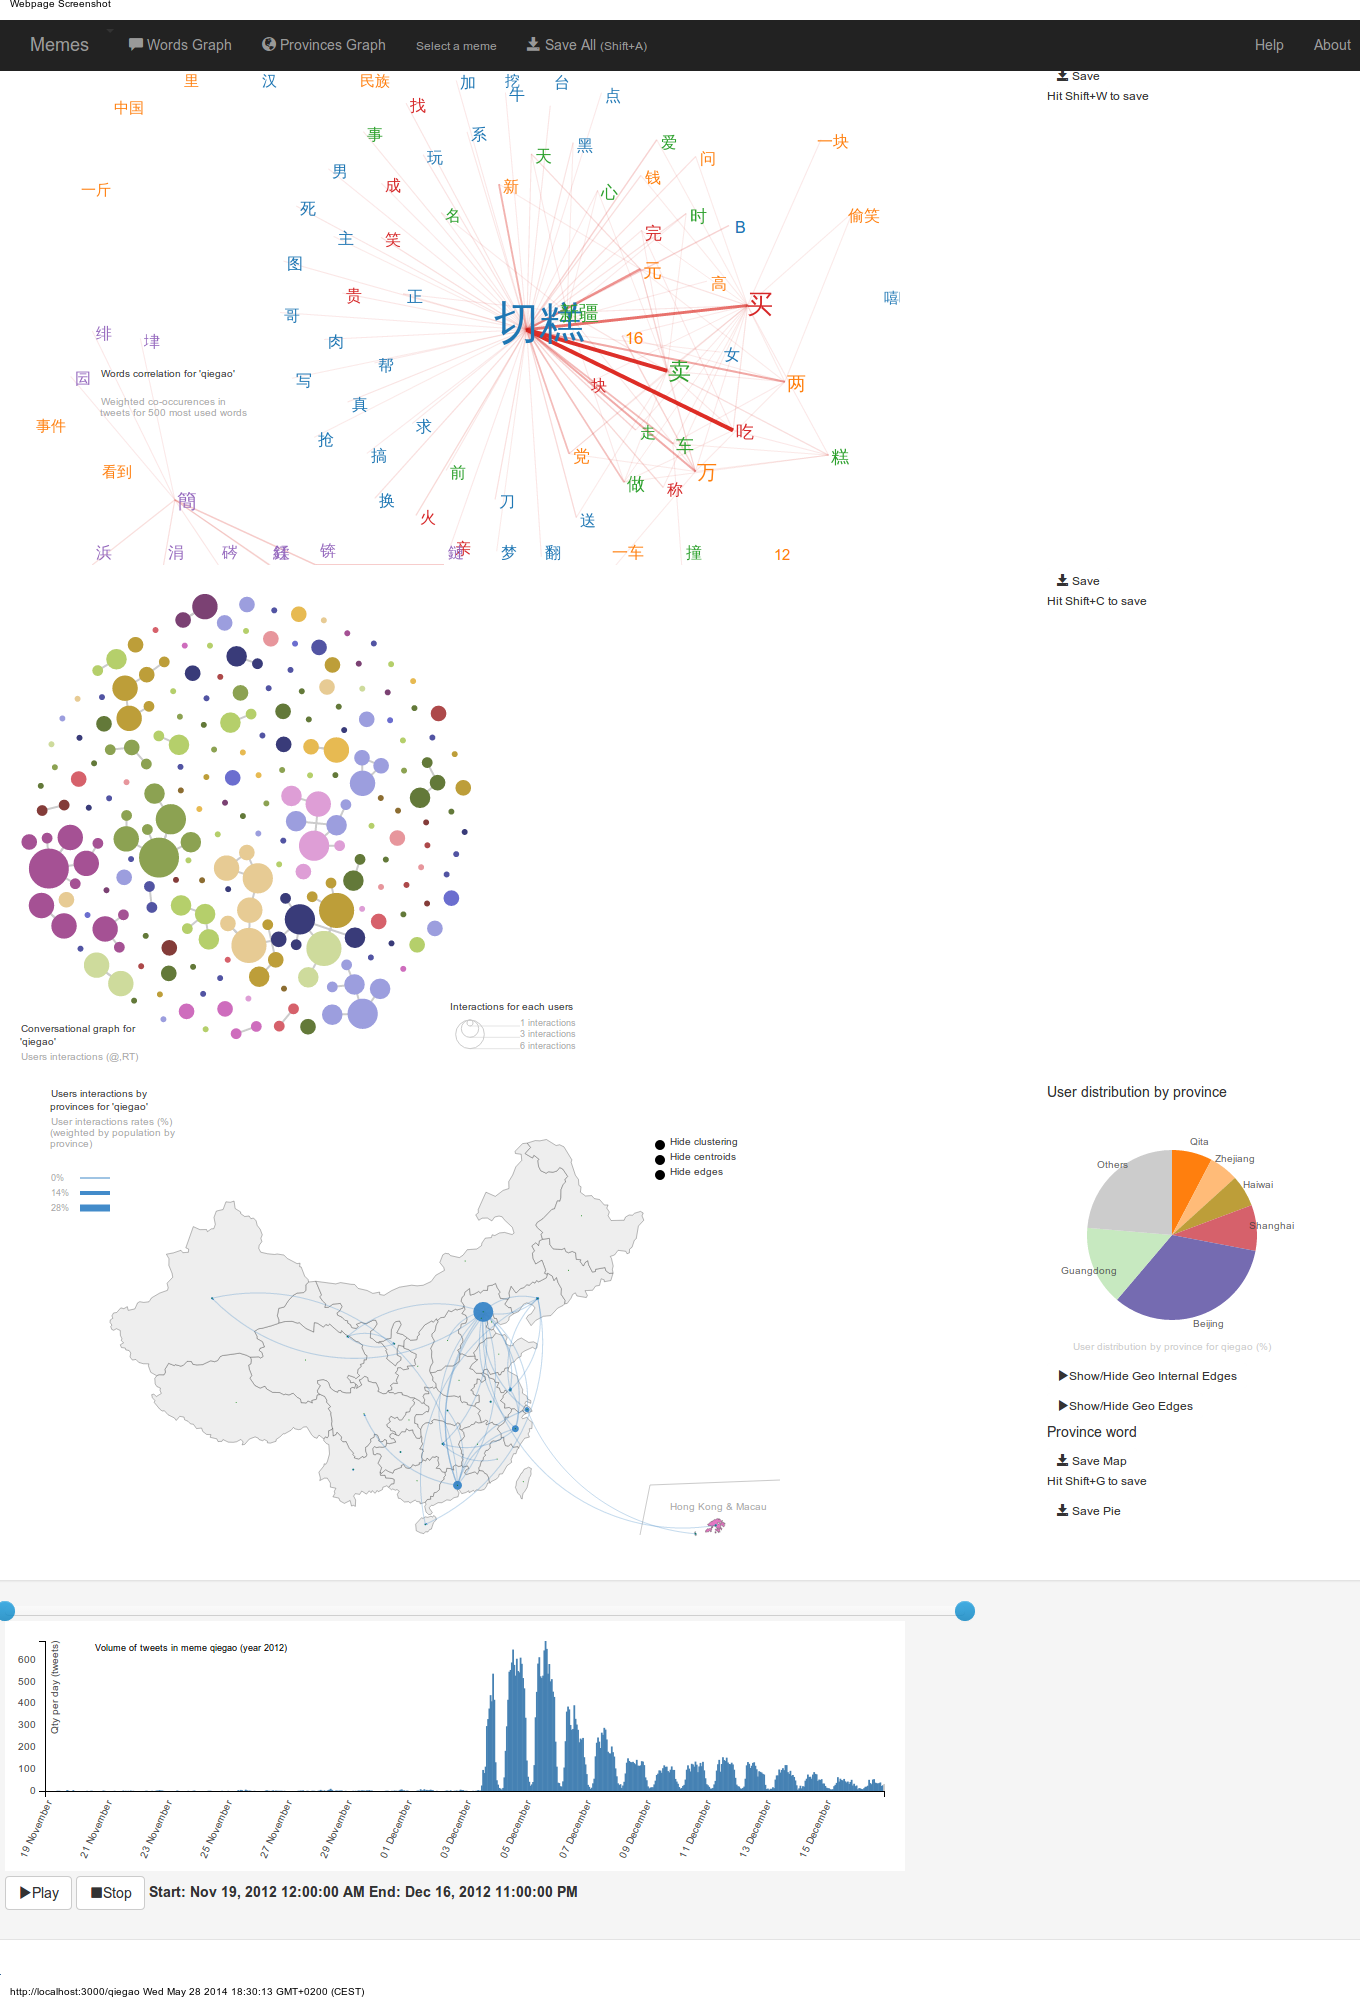
\includegraphics[width=6.7213in,height=8.3894in]{figures/chap4/ui/ui-screenshot.png}
    \caption{Interface d'exploration et de visualisation des données}
\end{figure}

\subsubsection{Organisation de l'espace visuel et perceptif}
\label{sec:viz}
    Devant la disparité des données en présence, nous devons donc construire un espace de représentation ou plut\^ot une interface de représentation propice à l{\textquoteright}exploration et la découverte des phénomènes dans les relations entre les différents graphes. Dans la définition de cet espace perceptif se joue la réconciliation d{\textquoteright}entités dissemblables (des utilisateurs, des lieux, des mots, leurs relations mutuelles). La t\^ache consiste à réconcilier dans le plan de l{\textquoteright}espace graphique de la visualisation (ici celui de l{\textquoteright}écran) les différents espaces o\`u projeter ces différents graphes. L'organisation de cet espace suppose tout d'abord une hiérarchisation de l'importance des contenus pour leur affichage. Ici, nous devons prendre en compte la nature des données affichées. La première décision est d'utiliser un défilement vertical qui permet de naviguer entre les différents graphes. Nous structurons l'espace en cinq parties clairement identifiées.


    \begin{figure}[h!]
        \label{fig:schema-viz}
        \centering

        \begin{tabular}{ | p{5cm} | p{2cm} | }
            \hline
            \multicolumn{2}{|c|}{Menu} \\[.3cm] 
            \hline
            Words  &         \\
            Semantic graph &  \\[.5cm] \cline{1-1}
            Users &  \\
            Conversational graph & Options\\[.5cm] \cline{1-1}
            Geo &  \\
            Map of China &  \\[.5cm] \cline{1-1}
            Time   & \\
            Timeline &  \\[.5cm]
            \hline 
        \end{tabular}
        \caption{Structure de l'interface d'exploration et de visualisation des données}
    \end{figure}


    Le centre de la visualisation est occupé par le réseau représentant les utilisateurs. En structurant l'espace autour des  utilisateurs, nous souhaitons montrer le r\^ole central des processus humains dans cette étude. Dans notre repr\'esentation, chaque utilisateur est un point et chaque interaction correspond \`a un trait. La couleur des points montre l{\textquoteright}appartenance de l{\textquoteright}utilisateur \`a une m\^eme communaut\'e de conversation calcul\'e gr\^ace \`a un algorithme de Louvain \citep{Blondel2008}. La taille des points expriment le nombre total de connexions entrantes et sortantes d{\textquoteright}un utilisateur. La distance entre les groupes d{\textquoteright}utilisateurs est d\'efinie en utilisant l{\textquoteright}algorithme \textit{force} de d3js \citep{Bostock2011} pour calculer leur r\'epulsion : plus les utilisateurs sont proches dans la conversation, plus les points les repr\'esentant sont proches dans le graphe. La forme circulaire du graphe est due aux propri\'et\'es physiques d{\textquoteright}attraction utilis\'ees lors du calcul qui permettent aux diff\'erents nodes du graphe de rester agr\'eger ensemble sans se diss\'eminer. Pour des questions de lisibilit\'e, seuls les 500 utilisateurs les plus actifs ont \'et\'e repr\'esent\'es. Les utilisateurs poss\'edant moins de deux interactions ont \'et\'e supprim\'es pour rendre le graphe lisible. 
    
    Le graphe de mots occupe lui la position haute. Éthérique et peu enraciné, la représentation de ce nuage sémantique trouve sa place dans le haut de l'espace visuel permettant de saisir d'un coup d’œil la teneur général des débats et de s'attarder sur les nœuds mystérieux créées dans le langage lors des conversations. Les graphes de mots pr\'esent\'es sont construits gr\^ace aux co-occurences de mots dans les messages. Si deux mots sont utilis\'es dans un m\^eme message, un \textit{edge} est ajout\'e entre eux, recr\'eant ainsi un graphe pond\'er\'e repr\'esentant une structure s\'emantique relationnelle d{\textquoteright}ensemble entre les mots. La taille des mots repr\'esente le nombre de fois o\`u il sont \'et\'e cit\'es dans l{\textquoteright}ensemble du corpus. Les couleurs d\'efinissent des communaut\'es de mots qui ont \'et\'e calcul\'ees gr\^ace \`a l{\textquoteright}algorithme de Louvain \citep{Blondel2008}. L{\textquoteright}\'epaisseur des traits repr\'esentent l{\textquoteright}intensit\'e des relations (leur nombre de co-occurences dans le corpus). La disposition des mots utilise \'egalement l{\textquoteright}algorithme Force de d3js \citep{Bostock2011} pour calculer la proximit\'e des mots sur la base de l{\textquoteright}intensit\'e de leurs relations. Afin de limiter la taille du graphe, nous avons s\'electionn\'e uniquement les 500 mots les plus utilis\'es.  


    La carte représentant la Chine, plancher des vaches, est positionnée en-dessous du graphe des utilisateurs (voir section suivante \ref{sec:le_temps_et_la_carte}). Enfin, l'axe temporel se situe tout en bas de la page, montrant le volume des conversations dans le temps. Sur la droite, un espace est laissé disponible pour permettre l'ajout de différentes options et l'affichage d'informations secondaires.
    

\subsubsection{Cartographie et visualisation interactive} 
\label{sec:le_temps_et_la_carte}
    
    La représentation des échanges entre les utilisateurs sur une carte géographique a présenté plusieurs difficultés. 

    La première étape a été de reconstituer une carte de la Chine par provinces comprenant également Taiwan, Hong Kong et Macau. Chacun de ces territoires possèdent une influence médiatique certaine en Chine et méritent à ce titre d{\textquoteright}être représenté. De plus, il était important de faire correspondre les informations géographiques disponibles dans le jeu de données (voir chapitre \ref{sec:geoloc}). Néanmoins, le statut politique particulier de chacun de ces territoires nous a obligé à reconstituer une carte o\`u ils figuraient tous. Nous avons pour ce faire utilisé les fichier Shapefile disponibles via \textit{Natural Earth} (Adminsitrative 1:10m)\footnote{\url{http://www.naturalearthdata.com/}, consulté le 9 Juillet 2014 à 10:42} pour constituer un seul et même fichier compatible au format \textit{geoJson} utilisant les noms standard \textit{ISO 3166-1 alpha-3} pour nommer les différents lieux.\footnote{Le détail des procédures utilisées ainsi que le code pour générer la carte sont disponibles à \url{https://github.com/clemsos/d3-china-map}, consulté le 9 Juillet 2014 à 10:41}. Nous avons choisi d{\textquoteright}aggrandir l{\textquoteright}échelle de Hong Kong et Macau en les mettant en exergue sur la droite de la carte afin qu{\textquoteright}il soit visible à l'échelle choisie pour le reste du territoire chinois. Egalement, nous avons choisi d'ignorer les données concernant les utilisateurs ayant choisi {\textquotedblleft}autres{\textquotedblright} ou {\textquotedblleft}reste du monde{\textquotedblright} comme leurs lieux de résidence dans leurs informations de profil. Ce choix a été motivé par notre réflexion sur l'Internet chinois  dans le cadre national et également linguistique (voir chapitre \ref{sec:internet-chine}).


    \begin{figure}
        \centering
        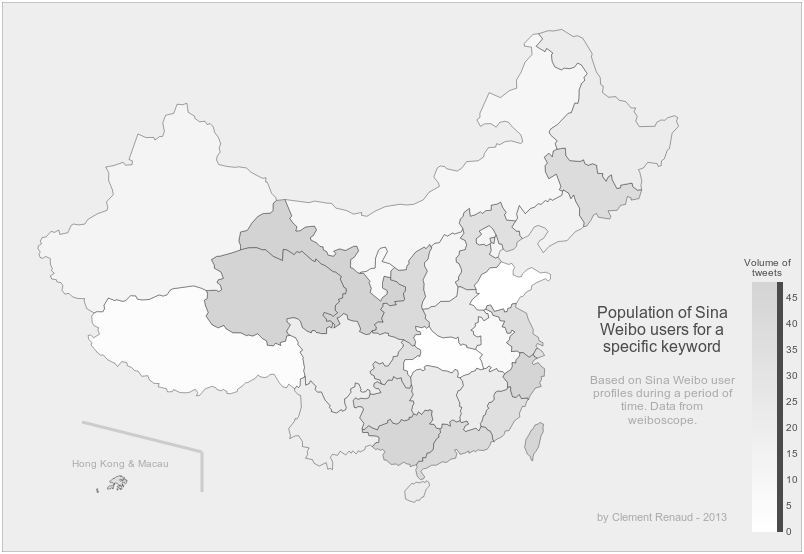
\includegraphics[scale=0.4]{figures/chap4/ui/ui-map.png}
        \caption{Carte interactive de la Chine (exemple contenant des données générées aléatoirement)}
        \label{fig:ui-map}
    \end{figure}

    La représentation des dynamiques entre province basée sur les échanges entre utilisateurs a également été le sujet de nombreuses réflexions. Nous avons pr\'ec\'edemment extrait pour chaque m\^eme le r\'eseau conversationnel des interactions entre utilisateurs. En associant chaque utilisateur \`a sa province d{\textquoteright}origine, \ nous pouvons reconstituer le r\'eseau des interactions entre provinces. 

    Afin de comprendre comment comment s{\textquoteright}agençaient spatialement chacune des discussions, nous avons d'abord choisi de représenter l{\textquoteright}ensemble des utilisateurs par province. Néanmoins, cette approche reflète essentiellement le nombre d'utilisateurs par ville, recréant bien souvent une carte des grandes villes contenant très peu d'informations. Pour faire face au biais de la carte, nous avons décidé de représenter les relations entre provinces sous formes d'une liste de noms reliées par des traits. La complexité de la figure rendait cette approche peu intéressante.

    Afin d{\textquoteright}observer comment les provinces s{\textquoteright}associent lors de la discussion, nous pr\'esentons le r\'eseau des interactions sous la forme d{\textquoteright}une graphe pond\'er\'e et dirig\'e. Pour des raisons de lisibilit\'e, les liens entre les provinces sont dirig\'es non pas vers la capitale de la province mais vers le \textit{centroid (barycentre) }de la forme g\'eom\'etrique qui la repr\'esente. Afin de r\'etablir un \'equilibre est de faire appara\^itre des dynamiques plus particuli\`eres, les r\'esultats ont \'et\'e pond\'er\'e par le pourcentage de population totale repr\'esent\'ee par chaque province dans le corpus utilis\'e (Weiboscope).

    Afin d{\textquoteright}explorer les différentes dimensions du graphes, nous avons également ajouté des interactions qui permettent de focaliser sur des zones ou des caractéristiques précises des graphes. Nous pouvons également exporter des graphes précis ou l'ensemble des graphes sous forme d'image qui peuvent être ensuite utilisés comme figures (voir \ref{sec:results-memes}). Nous avons mis en place des raccourcis claviers qui offrent notamment la possibilité de capturer des instantanés obtenus par la manipulation des graphes.
    
\subsubsection{Moteur de visualisation} 
\label{sec:moteur_de_visualisation}

    Les protocoles de communication entre base de données, serveur et affichage des graphes sont une des clés qui rendent possible la visualisation interactive. En effet, afin de pouvoir se concentrer sur des résultats ou des éléments spécifiques, il est nécessaire de pouvoir isoler un ensemble de données intéressants. L'utilisateur doit d'abord sélectionner un mème parmi ceux déjà traités existant dans la base de données. Il dispose d'un menu décrivant succinctement le mème par un titre et les mots clés utilisés lors de la recherche qui lui permettent de le reconnaître. En cliquant sur les boutons du menu, il accède à une page spécifique présentant le mème (voir figure \ref{fig:ui-menu}).

    \begin{figure}[h!]
        \centering
        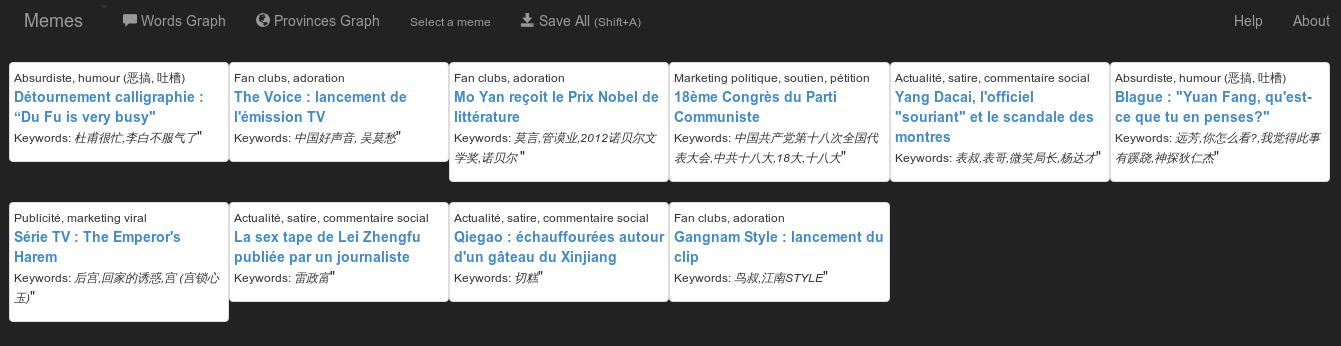
\includegraphics[scale=0.3]{figures/chap4/ui/ui-menu.png}
        \caption{Menu de sélection des mèmes}
        \label{fig:ui-menu}
    \end{figure}


    Une fois le mème affiché, l'utilisateur peut sélectionner les différentes parties qui l'intéressent. Une des caractéristiques importantes de ce logiciel est qu'il permet de choisir une période de temps à afficher. En déplaçant le curseur situé au dessus du graphe temporel, les données et leur affichage sont automatiquement mises à jour ce qui permet de se concentrer sur un temps de début et de fin. Afin de voir l'évolution sur une période donnée, un bouton \textit{play} permet d'animer automatiquement les graphes, montrant leurs évolutions sur la période de temps choisie (figure \ref{fig:ui-timeline}).

    \begin{figure}[h]
        \centering
        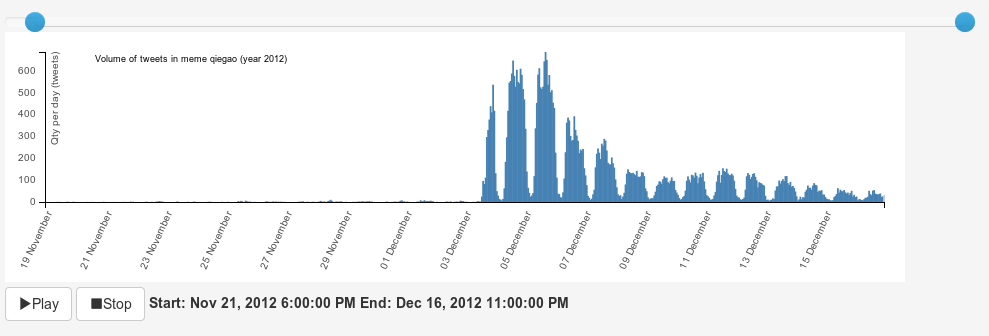
\includegraphics[scale=0.4]{figures/chap4/ui/ui-timeline.png}
        \caption{Cette timeline interactive permet de sélectionner une période de temps}
        \label{fig:ui-timeline}
    \end{figure}

    Pour obtenir cette fluidité dans l'interface, de nombreux composants doivent être synchronisés pour permettre 1) la communication avec la base de données, 2) l'obtention des données suivant la limite de temps et 3) la mise à jour de l'affichage. Pour ce faire, nous utilisons des technologies fondées sur le langage \textit{Javascript}. Le serveur chargé de communiquer avec la base de données est une application écrite en \textit{Node}\footnote{ \textit{"Node.js is a platform built on Chrome's JavaScript runtime for easily building fast, scalable network applications."} d'après url{http://nodejs.org/}, consulté le 8 Juillet à 15:05} qui est un framework généraliste de Javascript pour les serveurs. L{\textquoteright}ensemble de l{\textquoteright}outil de visualisation dans le navigateur se fonde sur HTML5, CSS3 et Javascript. La gestion des données dans le navigateur et la communication avec le serveur se fait grâce à la librairie \textit{AngularJS}\footnote{\textit{"HTML enhanced for web apps"} d'après\url{https://angularjs.org/}, consulté le 8 Juillet à 15:08}. Conçu par \textit{Google}, \textit{AngularJS} nous permet de standardiser et d'optimiser les fonctionnalités de traitement des données coté client. La visualisation des données utilise la librairie {\textquotedblleft}Data-Driven Documents{\textquotedblright} \citep{Bostock2011}\footnote{ D3js at \url{http://d3js.org/,} consulté le 24 Avril 2014 à 14:58}. L'interface des menus et boutons utilise le framework \textit{Bootstrap}\footnote{\textit{"Bootstrap is the most popular HTML, CSS, and JS framework for developing responsive, mobile first projects on the web."}, d'après \url{http://getbootstrap.com/}, consulté le 8 Juillet 2014 à 15:16}. L'ensemble du schéma de communication entre le serveur et le moteur de visualisation est disponibles dans les annexes de ce document (figure \ref{fig:ui-algo}).


    Nous avons fait ici le choix d'utiliser des technologies largement testées et reconnues parmi l'immensité des solutions disponibles. Ces frameworks et librairies possèdent déjà une grand fiabilité, étant utilisé en production par de très nombreux sites possèdant de grands nombre d'utilisateurs (comme Twitter pour Bootstrap ou Youtube pour Angular). La mise en place de ces framework permet également d'obtenir des résultats rapides lors des processus itératifs de prototypage. Enfin, l'usage d'outils déjà reconnus permet une meilleure lisibilité pour des utilisateurs ou ré-utilisateurs qui voudraient se saisir de cet outil.